\documentclass[11pt,a4paper]{article}

\usepackage[utf8]{inputenc}
\usepackage[T1]{fontenc}
\usepackage{libertinus}
\usepackage{libertinust1math}
\usepackage[english]{babel}
\usepackage{hyperref}
\usepackage{url}
\usepackage[dvipsnames]{xcolor}
\usepackage{microtype}
\usepackage{graphicx}
\usepackage{float}
\usepackage[margin=2.5cm]{geometry}

\hypersetup{
  colorlinks=true,
  linkcolor=blue!60!black,
  citecolor=blue!60!black,
  urlcolor=blue!60!black,
}

\title{\textbf{APIs We Built Are Meant for Computers:\\How Do We Expose Hypermedia APIs to LLMs?}}
\author{Antoine Bluchet\\\texttt{antoine@bluchet.fr}\\ORCID: \href{https://orcid.org/0009-0009-3597-2014}{0009-0009-3597-2014}
\and
K\'{e}vin Dunglas\\\texttt{kevin@dunglas.fr}\\ORCID: \href{https://orcid.org/0009-0000-3013-1384}{0009-0000-3013-1384}}
\date{}

\begin{document}

\maketitle

\begin{abstract}
Agent-based AI systems using protocols like the Model Context Protocol (MCP) separate ``application-controlled'' \texttt{Resources} (read-only context) from ``model-controlled'' \texttt{Tools} (callable actions). This paradigm is challenged by HATEOAS APIs such as those using the Hydra Core Vocabulary, where available actions are not static but discovered at runtime within resource content. The API expects the client to discover actions by reading content, but the MCP model is sandboxed and can only use predefined tools. We show that neither static endpoint-to-tool mapping nor a generic API-call tool preserves hypermedia discovery, and propose a \textbf{Dynamic Gateway Architecture} that resolves this mismatch. The gateway operates through three discovery phases---navigating the API entrypoint to give the agent a map of available collections, lazily registering typed CRUD and search tools when the agent visits a specific collection by cross-referencing its response with the API documentation (\texttt{docs.jsonld}), and honoring inline operation overrides that reflect per-resource state. A single static tool whose description embeds navigational guidance bootstraps the entire process without a system prompt. In a comparative evaluation against a static OpenAPI baseline (19~tasks, two models, $k{=}3$ runs), agents achieve 100\% task completion on all 15 positive-capability tasks ($n{=}90$ per condition), while the gateway reduces tool-schema overhead from 77\% to 2\% of input context---bridging the two protocols without violating the constraints of either.
\end{abstract}

\section{Introduction}

The field of applied artificial intelligence is shifting from monolithic models to agent-based systems. Protocols like the Model Context Protocol (MCP) support this shift by defining how an AI model interacts with external software~\cite{mcp-overview}. MCP's protocol defines two distinct capabilities: \texttt{Resources}, which are read-only data (e.g., files) controlled by the host \emph{application} to provide context to the model, and \texttt{Tools}, which are functions (e.g., \texttt{send\_email()}) controlled by the \emph{model} to perform actions~\cite{mcp-resources,mcp-tools}.

A gap emerges when attempting to connect AI agents to web APIs that follow the HATEOAS (Hypermedia as the Engine of Application State) constraint. These APIs are not static lists of functions. Systems like the Hydra Core Vocabulary define discoverable and state-dependent APIs~\cite{hydra}. Frameworks such as API Platform implement this vocabulary to produce fully hypermedia-driven web APIs~\cite{api-platform}. In a Hydra-powered API, an operation (e.g., \texttt{DELETE}) is not always available. It may only appear as an embedded \texttt{hydra:Operation} within a resource's content \emph{after} that resource has been fetched and \emph{if} the current user state permits it.

This creates an ``impedance mismatch'' based on a fundamental conflict between the operational models of the two protocols.

\begin{itemize}
  \item \textbf{The Hydra/HATEOAS Model:} This API design expects its client to be an active explorer. As described previously, an operation is a \textbf{content-based affordance}~\cite{hydra}. The client \emph{must} first \texttt{GET} a resource, \textbf{read} its content, and \textbf{discover} any available \texttt{hydra:Operation}s within that content before it can act. Actions are discovered at runtime within the resource's state.
  \item \textbf{The MCP Model:} This protocol imposes a ``sandbox'' on the AI model. The AI \emph{cannot} call \texttt{resources/read}; this is the responsibility of the ``application-controlled'' \texttt{resources} capability~\cite{mcp-resources}. The AI can \emph{only} call \textbf{predefined, list-based actions} from the ``model-controlled'' \texttt{tools} capability~\cite{mcp-tools}.
\end{itemize}

The mismatch is this: The Hydra API expects a client that \emph{discovers its actions by reading content}, but the MCP AI model is a client that \emph{cannot read content on its own} and \emph{can only use predefined actions}.

The research problem is: \textbf{How to bridge the gap between Hydra's content-based, state-dependent affordances and MCP's model-controlled, predefined \texttt{tool} paradigm?} This paper analyzes this mismatch, rejects two common integration models, and proposes a Dynamic Gateway Architecture that bridges the two protocols through lazy, navigation-triggered tool discovery.

\section{Analysis of Integration Models and Rejected Hypotheses}

Our final methodology was the result of a process of elimination, which disproved two initial hypotheses.

\subsection{The Static Tool-per-Endpoint Model}

Our first failed hypothesis was to treat MCP tools as direct, 1:1 mappings for traditional API endpoints. This approach can be seen in an experiment to add MCP support to the API Platform framework~\cite{api-platform-mcp}. The hypothesis is that the gateway can scan the API documentation (e.g., OpenAPI or Hydra's \texttt{ApiDocumentation}) at build-time and generate a static MCP \texttt{tool} for every available HTTP operation (e.g., \texttt{get\_recipes}, \texttt{post\_recipes}, \texttt{get\_recipe\_item}, \texttt{delete\_recipe\_item}).

By pre-generating all operations as static tools, the gateway breaks the HATEOAS constraint of discoverability. The tool list becomes a fixed snapshot of the API at build-time, unable to reflect state-dependent availability. An operation that should only appear when a resource is in a certain state (e.g., a \texttt{cancel} action on an active order) is exposed unconditionally, violating the principle that the server---not the client---controls which transitions are valid.

\subsection{The Single Generic Action Model}

The next hypothesis was to try a single, generic tool. The hypothesis is that an LLM can be given one tool like \texttt{call\_api(endpoint, method, payload)} and be instructed to parse the context to find the arguments. This model fails because it collapses navigation and mutation into one undifferentiated action. When a single tool handles both \texttt{GET} requests (whose primary purpose is discovery) and state-changing requests, the gateway has no structural hook to distinguish them: it cannot know when to intercept a response and extract affordances versus when to simply return a mutation result. The tool also requires the LLM to know the API's endpoints (\texttt{/recipes}, \texttt{/users}) and HTTP methods in advance to construct the first call---it provides no bootstrapping mechanism. The LLM does not have this a-priori knowledge; it is designed to \emph{discover} its options from its context. As we will show in our proposed architecture, separating navigation from mutation is essential: the navigation tool becomes the gateway's interception point for affordance discovery, while dynamically discovered typed tools handle state changes.

\section{Background and Positioning}

Fielding's REST dissertation introduced the HATEOAS constraint---that a client should discover available actions entirely through hypermedia controls embedded in server responses~\cite{fielding2000}. The Hydra Core Vocabulary~\cite{hydra} operationalizes this constraint for machine clients by encoding operations, property schemas, and link relations in JSON-LD. Despite two decades of REST, most recent work on LLM--API integration treats APIs as static function catalogs rather than navigable hypermedia systems.

Several lines of work have explored how LLMs can invoke tools and APIs. Some bake a fixed tool set into the model itself---Toolformer~\cite{schick2023toolformer} trains an LLM to self-supervisedly insert calls to a small, predetermined repertoire of tools during generation. Others scale the catalog: AnyTool~\cite{du2024anytool} introduces a hierarchical agent that retrieves from 16,000+ pre-indexed API descriptions, but ``discovery'' remains a search over a static index, not an extraction from API responses. RestGPT~\cite{song2023restgpt} chains RESTful API calls via a planning module but requires an upfront OpenAPI specification to enumerate all available endpoints. Benchmarks such as API-Bank~\cite{li2023apibank} evaluate tool-use capabilities against a fixed set of 73~API tools. The common thread is the assumption of a \emph{static, pre-indexed API catalog}: the set of available operations is available to the system before the interaction begins. None of these designs address runtime-discovered, state-dependent affordances---the distinguishing characteristic of HATEOAS APIs.

We do not empirically compare against these systems---they address a different problem (selecting from known APIs), not runtime affordance discovery. Our empirical comparison (Section~5) evaluates against a static OpenAPI baseline, the natural counterpart for the same API.

\section{The Dynamic Gateway Architecture: A Proposed Solution}

The analysis of these failed models led to our proposed solution: a \textbf{Dynamic Gateway Architecture}. The design is governed by two constraints: the AI model remains sandboxed---it can only call \texttt{tools}, not \texttt{resources/read}~\cite{mcp-tools}---and the gateway cannot have a static, hardcoded list of endpoints; it must discover operations by navigating hypermedia controls~\cite{hydra}. The architecture consists of one static tool and a set of dynamically discovered tools, connected by a multi-phase discovery process illustrated in Figure~\ref{fig:discovery}.

\subsection{The Static ``Navigation'' Tool}

A single static tool is defined that is always available. This tool enables the AI to perform HATEOAS navigation and is the gateway's sole interception point for affordance discovery.

\begin{itemize}
  \item \textbf{Tool:} \texttt{read\_api\_resource(uri)}
  \item \textbf{Purpose:} This tool allows the AI to request that the application fetch a resource (a \texttt{GET} request) and place its content into the context for the \emph{next} turn. Its purpose is to \emph{learn, navigate, and discover}.
  \item \textbf{Mechanism:} When the AI model sees a link in its context (e.g., a URI for \texttt{book} in an \texttt{Entrypoint}), it can call \texttt{read\_api\_resource(uri: "/books")}. The \emph{implementation} of this tool on the gateway is what triggers the dynamic discovery process described in Section~4.2. This is the only tool the agent starts with; all other tools are discovered dynamically.
\end{itemize}

\subsection{The Dynamic ``Discovery'' Process (Triggered by Navigation)}

The core of our architecture is the process triggered by the \texttt{read\_api\_resource} tool. Discovery operates through three phases, each corresponding to a distinct moment in the agent's interaction with the API.

The Hydra specification defines operations at two levels~\cite[§5]{hydra}:

\begin{enumerate}
  \item \textbf{Class-level operations} (\texttt{hydra:supportedOperation} on \texttt{hydra:supportedClass} inside \texttt{docs.jsonld}): These describe operations that all instances of a given type support---e.g., \texttt{POST} on a collection to create a resource, or \texttt{DELETE} on an item. As the specification states, ``all instances of a specific class typically support the same operations.'' These are type-scoped and do not change per-resource.
  \item \textbf{Instance-level operations} (\texttt{hydra:operation} inline in a resource response): These are state-dependent overrides---e.g., an order that can no longer be cancelled removes its \texttt{DELETE} operation. In current practice, some frameworks (e.g., API Platform) describe operations exclusively in \texttt{docs.jsonld} and do not embed them inline in responses, but the architecture must not assume this---any Hydra API may use inline operations to express per-instance state.
\end{enumerate}

The gateway's three-phase discovery strategy maps directly onto these levels, plus the collection-specific affordances (\texttt{hydra:search}) that Hydra provides inline.

\begin{figure}[H]
  \centering
  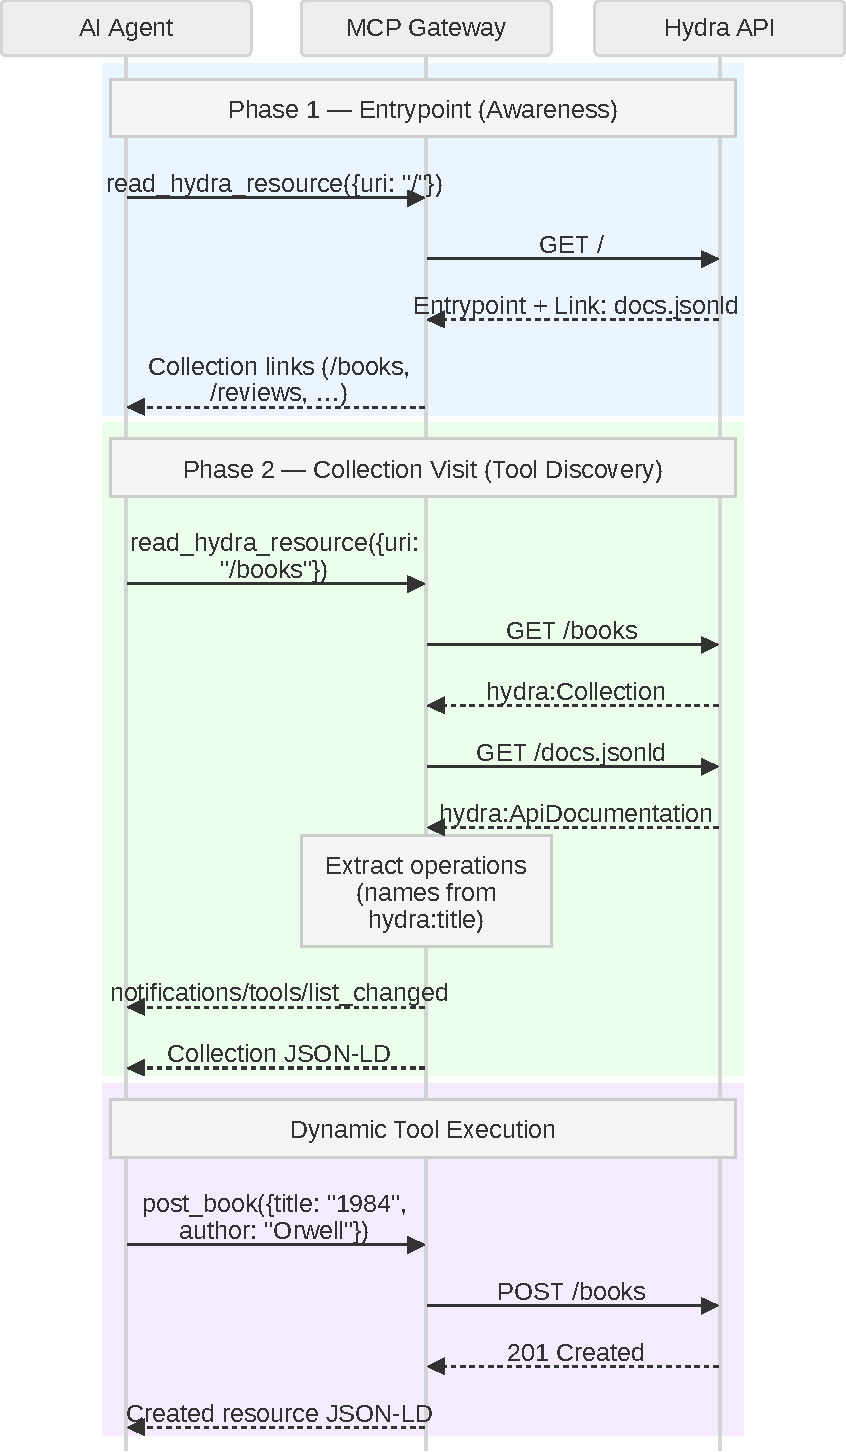
\includegraphics[width=0.85\linewidth]{diagram-sequence.pdf}
  \caption{The three-phase discovery process. Phase~1 gives the agent awareness of available collections. Phase~2 triggers tool registration (named from \texttt{hydra:title}) when a collection is visited. Phase~3 handles inline operation overrides for instance-level state. The final exchange shows a dynamically discovered tool being used for a mutation.}
  \label{fig:discovery}
\end{figure}

\subsubsection{Phase~1: Entrypoint Navigation (Awareness)}

When the AI first calls \texttt{read\_api\_resource(uri: "/")}, the gateway fetches the entrypoint. This response contains the map of the API---links to each available collection (e.g., \texttt{"book":"/books"}, \texttt{"bookmark":"/bookmarks"})---but \textbf{no tools are registered at this stage}. The gateway also inspects the HTTP \texttt{Link} header for the \texttt{http://www.w3.org/ns/hydra/core\#apiDocumentation} relation, which points to the \texttt{docs.jsonld} document, and caches its URL for later use.

The entrypoint gives the agent \emph{awareness}---it knows what collections exist and can plan which to visit---but not yet \emph{capabilities}. The agent's only tool remains \texttt{read\_api\_resource}. This separation is deliberate: registering tools for all resource types at this stage would consume significant tokens in the model's context on every turn, regardless of whether the agent ever interacts with those resources.

\subsubsection{Phase~2: Collection Navigation (CRUD and Search Discovery)}

When the agent navigates to a specific collection, the gateway performs the core discovery step: it identifies the collection's managed class from the response, fetches \texttt{docs.jsonld}, and registers typed tools for that class's operations. We illustrate this with an example.

The AI's context now contains:

\begin{small}
\begin{verbatim}
{"@context":"/contexts/Entrypoint","@id":"/","@type":"Entrypoint",
 "book":"/books",...}
\end{verbatim}
\end{small}

If the user asks, ``Show me the books,'' the AI model sees the \texttt{"book":"/books"} link in its context. It calls:

\begin{small}
\begin{verbatim}
tools/call(name: "read_api_resource",
           arguments: { "uri": "/books" })
\end{verbatim}
\end{small}

When the \textbf{MCP Gateway} executes this tool, it proxies the \texttt{GET /books} request to the Hydra API, then performs two extraction steps on the response:

\textbf{Managed class resolution.} The gateway identifies the type of resources the collection manages. It first checks for a \texttt{hydra:memberAssertion} declaring the \texttt{rdf:type} of members~\cite[§6]{hydra}. If absent, it falls back to dereferencing the collection's \texttt{@context} URL (e.g., \texttt{/contexts/Book}) to resolve the class IRI from the vocabulary base.

\textbf{Operation extraction.} Once the managed class is known (e.g., \texttt{Book}), the gateway fetches \texttt{docs.jsonld} and extracts operations from two locations, following the Hydra specification's distinction between class-level and link-level operations~\cite[§5]{hydra}: the class's own \texttt{hydra:supportedOperation} entries (item-level operations) and the \texttt{Entrypoint} class's \texttt{supportedProperty} entries whose range targets the managed class (collection-level operations such as \texttt{POST}). Each operation carries its own name via \texttt{hydra:title} (e.g., \texttt{postBook}, \texttt{deleteBook}). The gateway uses this name directly---converted to snake\_case---as the MCP tool name, rather than inferring semantics from the HTTP method. This preserves custom operation names (e.g., \texttt{cancelOrder} $\to$ \texttt{cancel\_order}) without any mapping heuristic. Input schemas for write operations are built from the writable \texttt{hydra:supportedProperty} entries of the operation's \texttt{expects} class; item-level tools include a \texttt{uri} parameter so the agent can specify which resource to act on. The gateway also extracts \texttt{hydra:search} blocks from the collection response and registers them as search tools.

If new tools were created, the gateway sends a \texttt{notifications/tools/list\_changed} message~\cite{mcp-tools} and returns the collection content to the agent. Crucially, tools for other resource types remain unregistered until the agent navigates to their respective collections---the tool set grows proportionally to the task scope, not to the API's total surface area.

\subsubsection{Phase~3: Inline Operation Overrides (Instance-Level State)}

When the agent navigates to a specific resource or collection and the response contains \texttt{hydra:operation} nodes, the gateway registers these as tools that may differ from---or supplement---the class-level defaults discovered in Phase~2. For example, if a fetched order resource includes only \texttt{GET} and \texttt{PATCH} in its inline \texttt{hydra:operation}---omitting \texttt{DELETE}---an implementation could choose to remove or disable the \texttt{delete\_order} tool, reflecting the server's assertion that deletion is not available in the current state. The design anticipates that inline operations are authoritative; how exactly the tool set is reconciled (additive registration, replacement, or removal) is an implementation decision.

This phase is the most faithful to the HATEOAS principle: the server communicates exactly which transitions are valid for \emph{this} resource in \emph{this} state, and the gateway translates that signal into the agent's available tool set. Inline operations take precedence over class-level defaults because they represent the server's authoritative, state-dependent view. This phase is architecturally defined but has not yet been validated empirically; the evaluation in Section~5 exercises only Phases~1 and~2.

\medskip

Across all three phases, the same principle applies: Hydra's \texttt{hydra:supportedOperation} and \texttt{hydra:IriTemplate} (\emph{content-based} affordances) are translated into MCP \texttt{tools} (\emph{action-based} affordances), making them available to the AI only after they have been discovered.

\subsection{Illustrative Interaction}

To demonstrate the architecture in practice, we present a condensed agent transcript from our prototype connected to a Hydra API serving a book catalog (76 books, with search filters). No system prompt is provided---the agent's only guidance is the static tool's description: ``Navigate to a Hydra API resource by URI. Returns JSON-LD content and may discover new tools from hypermedia controls. Use this to explore the API: start with \texttt{"/"} to see the entrypoint, then follow links.''

The user asks: ``Could you check if there's a book by Orwell in our Hydra API?'' The agent proceeds as follows:

\begin{enumerate}
  \item \textbf{Phase~1:} The agent calls \texttt{read\_api\_resource(uri: "/")} and receives the entrypoint, learning that \texttt{/books} exists.
  \item \textbf{Phase~2:} The agent calls \texttt{read\_api\_resource(uri: "/books")}. The gateway resolves the managed class (\texttt{Book}), fetches \texttt{docs.jsonld}, and registers \texttt{post\_book}, \texttt{get\_book}, \texttt{patch\_book}, \texttt{delete\_book}, and \texttt{search\_books}. The agent receives the collection and notices the search filter.
  \item \textbf{Search:} The agent calls the newly discovered \texttt{search\_books(author: "Orwell")} tool and finds one result: ``The Lion and the Unicorn'' by George Orwell.
\end{enumerate}

The user then asks to add another Orwell book. The agent---now equipped with the \texttt{post\_book} tool discovered in step~2---calls it directly with the appropriate fields, successfully creating the resource in a single tool call. At no point was the agent given prior knowledge of the API's schema, field names, or available operations; in our evaluation, the tool description proved sufficient to bootstrap discovery, and everything else was learned through navigation.

\section{Evaluation}

To validate the dynamic gateway architecture, we conducted a comparative evaluation against a static OpenAPI baseline. We measured task completion rates, token consumption, and tool-schema overhead across 19~tasks of increasing complexity, using two LLMs via the same MCP client.

\subsection{Setup}

We evaluate two conditions:

\begin{itemize}
  \item \textbf{Condition~A (Hydra gateway):} Our dynamic gateway, starting with one static tool (\texttt{read\_api\_resource}) and lazily discovering typed tools at runtime.
  \item \textbf{Condition~B (OpenAPI static):} A conventional MCP server generated from the same API's OpenAPI specification, exposing all 19~operations as pre-registered tools from the start.
\end{itemize}

Both conditions connect to the same upstream API: a Hydra-powered book catalog built with API Platform, seeded with 76~books across multiple authors, with reviews as sub-resources, bookmarks, parchments, and users. The API exposes search filters on title, author, and condition. Each run resets the database to a deterministic fixture state before execution.

We use two models---Gemini~2.5~Flash and GPT-5~mini---accessed through the OpenCode CLI (GitHub Copilot) in headless mode, with 3~runs per task per model per condition. Neither condition uses a system prompt. Under Condition~A, the static tool's own description (``Navigate to a Hydra API resource by URI\ldots{} start with \texttt{"/"} to see the entrypoint, then follow links'') provides sufficient guidance for the agent to bootstrap discovery without additional instructions.

\subsection{Task Design}

The 19~tasks are organized into four tiers of increasing difficulty. Full task definitions are given in Appendix~\ref{appendix:tasks}.

\begin{itemize}
  \item \textbf{Tier~1 --- Single-resource read} (5~tasks): Retrieving information from the collection or a specific resource. Includes one negative-capability task (T1.5) asking for a filter the API does not support.
  \item \textbf{Tier~2 --- Single mutation} (6~tasks): Creating, updating, or deleting a resource via a single operation. Includes two negative-capability tasks (T2.5, T2.6) testing whether the agent recognizes missing or read-only fields.
  \item \textbf{Tier~3 --- Multi-step reasoning} (4~tasks): Tasks requiring multiple navigations and operations---e.g., searching by author, then updating each result's condition.
  \item \textbf{Tier~4 --- Cross-collection and discovery stress} (4~tasks): Operations spanning multiple collections or requiring extensive exploration. Includes one negative-capability task (T4.4) testing whether users are read-only.
\end{itemize}

Goals are evaluated automatically: \texttt{api\_state} goals verify the database state via HTTP after the run; \texttt{response\_contains} and \texttt{response\_indicates\_limitation} goals check the agent's textual output against expected keywords.

\subsection{Results}

\subsubsection{Task Completion}

Table~\ref{tab:completion} summarizes pass rates by tier and condition.

\begin{table}[H]
\centering
\small
\begin{tabular}{l|cc|cc}
\hline
 & \multicolumn{2}{c|}{\textbf{Condition~A (Hydra)}} & \multicolumn{2}{c}{\textbf{Condition~B (OpenAPI)}} \\
\textbf{Tier} & Gemini & GPT-5-mini & Gemini & GPT-5-mini \\
\hline
1 --- Read         & 80.0\% & 86.7\% & 84.0\% & 80.0\% \\
2 --- Mutation     & 94.4\% & 88.9\% & 96.7\% & 100.0\% \\
3 --- Multi-step   & 100.0\% & 100.0\% & 100.0\% & 100.0\% \\
4 --- Cross-coll.  & 91.7\% & 75.0\% & 80.0\% & 75.0\% \\
\hline
\textbf{Overall}   & \textbf{91.2\%} & \textbf{87.7\%} & 90.5\% & 89.5\% \\
\hline
\end{tabular}
\caption{Pass rates by tier and condition ($k=3$ runs per task per model).}
\label{tab:completion}
\end{table}

On \textbf{positive-capability tasks} (15~tasks excluding negative-capability tests), both models achieve \textbf{100\%} pass rate under both conditions ($n{=}90$ runs per condition)---every CRUD operation, search, multi-step workflow, and cross-collection task succeeds in all runs.

The overall gap is driven entirely by \textbf{negative-capability tasks}, where the agent must recognize that an operation is impossible and report a limitation rather than attempting it. These tasks are inherently difficult for both conditions: T1.5 (no publication-year filter) achieves 0--33\% across all configurations; T4.4 (read-only users) is 0--67\%. Negative capability is a model-level challenge, not an architectural one.

\subsubsection{Token Consumption and Schema Overhead}

On this 19-operation API, Condition~A uses approximately 2$\times$ more total tokens than Condition~B per task, driven by navigation overhead: the agent must first read the entrypoint and a collection before acting, adding 2--3~tool calls to every task.

However, the \emph{composition} of token usage differs dramatically. We estimate tool-schema overhead---the tokens consumed by injecting tool definitions into the model's context on each turn---using the measured tool counts per turn:

\begin{itemize}
  \item \textbf{Condition~B:} All 19~tool schemas (~1,685~tokens) are injected into every turn, consuming a mean of \textbf{77.2\%} of input tokens on schema alone.
  \item \textbf{Condition~A:} Starting with 1~tool (~51~tokens) and growing lazily, schema overhead is a mean of \textbf{2.0\%} of input tokens.
\end{itemize}

This overhead scales linearly with API size. For a 200-operation API, Condition~B would inject approximately 17,800~schema tokens per turn regardless of the task, while Condition~A would still begin at~51 and only load the tools the agent actually needs. The gateway's lazy discovery ensures that context budget is spent on task-relevant data rather than unused tool definitions---and as API size grows, the static baseline's per-turn schema cost eventually exceeds the gateway's navigation overhead, inverting the token trade-off.

\subsubsection{Discussion}

The evaluation demonstrates that dynamic hypermedia-driven discovery achieves task-completion parity with a static OpenAPI baseline, while fundamentally changing how context is allocated. The Hydra gateway trades upfront navigation cost (2--3~extra tool calls) for a tool set that scales with task scope rather than API surface area. The architecture relies on the MCP \texttt{notifications/tools/list\_changed} mechanism; correct client-side handling of this notification is essential for dynamic discovery to function.

One design asymmetry is worth noting: Condition~A's single tool description encodes navigational guidance (``start with \texttt{"/"}\ldots{} then follow links''), while Condition~B's tool descriptions are individual operation schemas with no comparable framing. This reflects a genuine difference in how the two approaches convey interface semantics, not an experimental confound.

The MCP specification defines an optional \texttt{instructions} field in the server's initialization response, which clients \textsc{may} inject into the model's system prompt~\cite{mcp-overview}. Our gateway defines such instructions---a workflow (``navigate first, then act'') and rules (``never guess URIs or field values; reuse exact values from responses'')---but the evaluation client (OpenCode) does not honor this field. All reported results reflect the tool description alone.

\subsubsection{Threats to Validity}

\textbf{Internal.} All tasks were evaluated against a single Hydra API (a book catalog). The API does not exercise Phase~3 inline operation overrides in its current configuration---all operations are class-level. Phase~3 remains an architectural proposal validated only by design analysis, not by empirical evidence. Results may differ for APIs with state-dependent per-instance operations. The 3-run sample size per task limits statistical power; observed pass rates on negative-capability tasks are noisy.

\textbf{External.} We tested two models from different providers. Results may not generalize to models with weaker tool-calling or instruction-following capabilities. The evaluation uses a single MCP client (OpenCode); other clients may handle \texttt{tools/list\_changed} notifications differently, affecting discovery reliability.

\textbf{Construct.} Token overhead estimates for Condition~B use a fixed per-tool token count measured from the actual OpenAPI MCP server. The 200-operation extrapolation assumes linear scaling, which holds for tool schemas but may not account for model-level context management strategies (e.g., tool summarization).

\section{Conclusion}

In our evaluation, AI agents interacted with a hypermedia API as effectively as with static OpenAPI endpoints---achieving \textbf{100\%} task completion on all 15 positive-capability tasks across two models ($k{=}3$ runs per task, $n{=}90$ per condition) while reducing tool-schema overhead from 77\% to 2\% of input context, with no system prompt required.

The key architectural insight---separating navigation from mutation so that the tool set grows with task scope---yields a 38$\times$ reduction in schema overhead (from 77\% to 2\% of input context) at the cost of 2--3 additional navigation calls per task.

The main limitation is navigation overhead: the agent must visit the entrypoint and a collection before acting, roughly doubling total token consumption compared to the static baseline on this 19-operation API. However, this overhead is fixed per collection visited, while the static baseline's schema cost scales linearly with API size---for sufficiently large APIs, the dynamic approach becomes more token-efficient overall. The architecture also depends on correct client-side handling of \texttt{notifications/tools/list\_changed}, which not all MCP clients may implement reliably.

Phase~3 (inline operation overrides) is architecturally defined but unvalidated; testing against APIs with state-dependent per-instance operations is the most immediate priority for future work. Additional directions include evaluating with a broader set of models and measuring the crossover point at which lazy discovery becomes more token-efficient than static tool injection.

\bibliographystyle{unsrturl}
\bibliography{references}

\appendix

\section{Evaluation Task Definitions}
\label{appendix:tasks}

Table~\ref{tab:tasks} lists all 19~evaluation tasks. Tasks marked with~$\dagger$ are negative-capability tests where the expected outcome is that the agent reports a limitation. Goal types: \textbf{RC}~= response contains keywords; \textbf{RL}~= response indicates limitation; \textbf{AS}~= API state verified via HTTP; \textbf{ASC}~= chained API state (multi-step HTTP verification).

\begin{table}[H]
\centering
\small
\begin{tabular}{clp{7.2cm}l}
\hline
\textbf{ID} & \textbf{Tier} & \textbf{Prompt (abbreviated)} & \textbf{Goal} \\
\hline
T1.1 & 1 & Is there a book by Dan Simmons? & RC \\
T1.2 & 1 & What is the rating of `Hyperion'? & RC \\
T1.3 & 1 & Show all books by Gordon R.\ Dickson. & RC \\
T1.4 & 1 & How many reviews does `Hyperion' have? & RC \\
T1.5$^\dagger$ & 1 & Find all books published after 2000 (API only). & RL \\
\hline
T2.1 & 2 & Add a book with Open Library ID OL1168083M, condition `new'. & AS \\
T2.2 & 2 & Delete `Dragons of Deltora' by Emily Rodda. & AS \\
T2.3 & 2 & Change the condition of `Hyperion' to `new'. & AS \\
T2.4 & 2 & Write a review for `Hyperion': ``A masterpiece\ldots'', rating~5. & ASC \\
T2.5$^\dagger$ & 2 & Add a book `Brave New World' by Aldous Huxley. & RL \\
T2.6$^\dagger$ & 2 & Change the author of `Hyperion' to `Daniel Simmons'. & RL \\
\hline
T3.1 & 3 & Find all books by Vera Strange, update their condition to `new'. & AS \\
T3.2 & 3 & Check if Philip F.\ Nowlan exists; if not, add OL37044569M. & RC \\
T3.3 & 3 & Find `Hyperion', read its reviews, report the highest-rated. & RC \\
T3.4 & 3 & Bookmark `Hyperion'. & RC \\
\hline
T4.1 & 4 & List all available collections. & RC \\
T4.2 & 4 & Add book OL35227850M (new), then write a review for it. & AS \\
T4.3 & 4 & Search books by Gordon R.\ Dickson, summarize reviews. & RC \\
T4.4$^\dagger$ & 4 & Create a new user named `Alice'. & RL \\
\hline
\end{tabular}
\caption{Evaluation tasks by tier. $\dagger$~= negative capability (agent should report limitation).}
\label{tab:tasks}
\end{table}

\section{Evaluation Protocol}
\label{appendix:protocol}

Each evaluation run follows a deterministic protocol:

\begin{enumerate}
  \item \textbf{Fixture reset:} The upstream API database is reloaded with a fixed seed (\texttt{FIXTURES\_SEED=42}, 76~books), ensuring identical starting state across all runs.
  \item \textbf{MCP session cache cleared:} Any persisted affordance state from prior runs is removed.
  \item \textbf{Agent execution:} The MCP client (OpenCode) is launched in headless mode with the task prompt, a 120-second timeout, and the target model. No system prompt is used in either condition.
  \item \textbf{Gateway logging:} The MCP gateway logs all request/response pairs as NDJSON, capturing tool call sequences, tool-list snapshots at each \texttt{tools/list} exchange, and error events.
  \item \textbf{Goal evaluation:} Goals are checked automatically after the run completes. \texttt{api\_state} goals issue HTTP requests to the upstream API and verify response fields; \texttt{response\_contains} and \texttt{response\_indicates\_limitation} goals match the agent's textual output against keyword lists.
  \item \textbf{Result persistence:} Each run produces a JSON file containing the prompt, full response, token usage, tool call trace, gateway metrics, and goal evaluation result.
\end{enumerate}

The analyzer script re-evaluates text-based goals offline against current task definitions, allowing keyword lists to be refined without re-running experiments. API-state goals retain their original (baked) evaluation since the database state is ephemeral.

\end{document}
